\documentclass[letterpaper]{article}

\newcommand{\sect}[1]{\begin{center}\textbf{#1}\end{center}}
\usepackage[numbers]{natbib}
\usepackage{graphicx}
\usepackage{subcaption}
\usepackage{float}
\graphicspath{{./Images/}}

\begin{document}

\sect{Data}

\section{Introduction}

For this project we need needed various layers of GIS Data that would form important features necessary 
for identification of suitable locations for solar farms. Terrain information is a really important feature
for this study because for setting up a solar farm we require large tracts of land with little changes in
elevation. Solar irradiance is another important feature to be considered, Solar irradiance is defined as 
the amount of energy that could be generated from solar radiation incident on that certain place it is 
measured in watts per meter square $W/m^2$. Other important factors to consider are land cost, population
density, land use, protected wildlife sanctuaries, etc.

\section{Terrain Data}

United States Geological Survey (USGS) is an agency of United States government that works across disciplines
like geology, geography and hydrology. SRTM (Shuttle Radar Topography Mission) was undertaken to created 
digital elevation models (DEM) of earth surface in collaboration with NASA (National Aeronautics and Space
Agency). This resulted in two Digital Elevation Models available for research with spatial resolutions of 
1 arc-second (~30 meters) and 3 arc-second (~90 meters). For this study we will be using the DEM model with
1 arc second of spatial resolution\cite{USGS}.


\subsection{How to Access Data}

The Data is hosted on OpenTopography as a data collection\cite{OpenTopography}. It can be accessed via 
OpenTopography API after setting up an account. The data is hosted on a AWS S3 bucket in a linear file 
structure with many data files of '.tif' format. These are raster files that contain a raster band for
elevation data with data value in meters. The files are named with corresponding latitude and longitude
that helps in indentification of corresponding land area. 

\subsection{Data preparation and visualisation}

We can use GDAL library\cite{GDAL} from Open Source GeoSpatial Foundation for reading the raster layers 
from '.tif' files and extracting the terrain data and visualising it.


\begin{figure}[H]
    \centering
    \begin{subfigure}{0.49\textwidth}
        \centering
        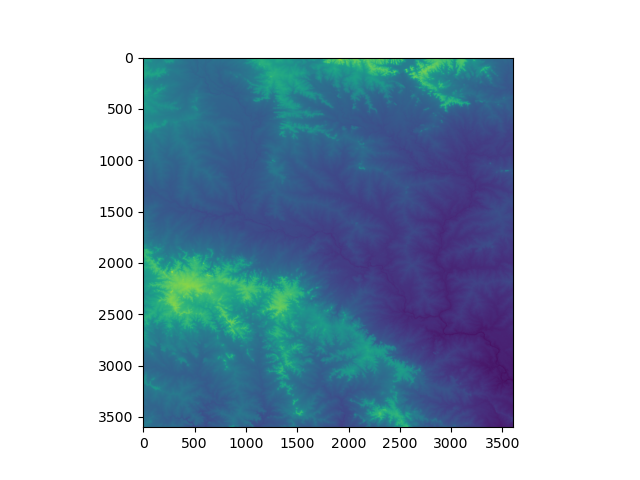
\includegraphics[width=1\textwidth]{Elevation}
        \caption{Elevation map for coordinates N 20' E 78'}\label{fig:Elevation}
    \end{subfigure}
    \hfill
    \begin{subfigure}{0.49\textwidth}
        \centering
        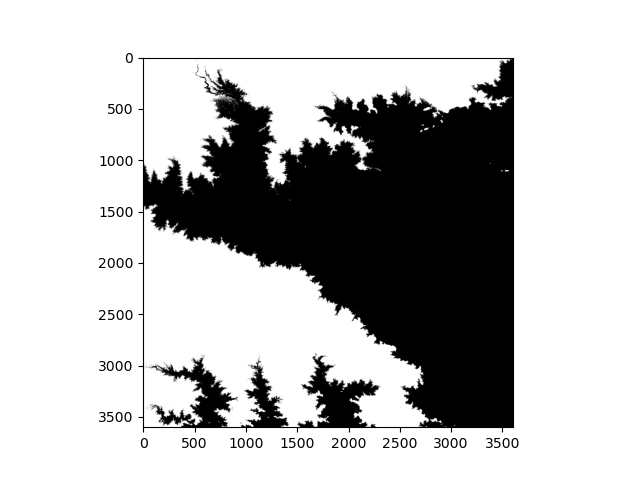
\includegraphics[width=1\textwidth]{Mask}
        \caption{Elevation values with a mask on average}\label{fig:elevation-mask}
    \end{subfigure}
    \caption{Comparison of Elevation and Elevation Data}
\end{figure}

\begin{figure}[H]
    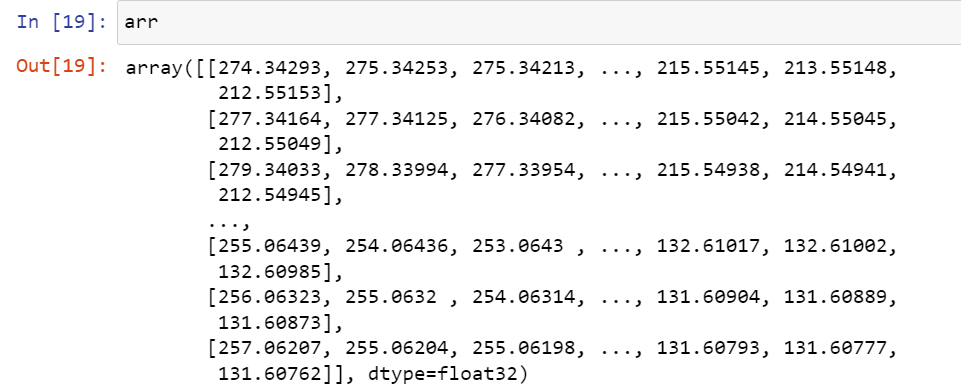
\includegraphics[width=0.7\textwidth]{ElevationData}
    \caption{Elevation values for coordinates N 20' E 78' in meters}
    \centering
\end{figure}



\section{Solar Irradiance Data}

National Solar Irradiance Database (NSRDB)\cite{Sengupta_Xie_Lopez_Habte_Maclaurin_Shelby_2018} is a database of solar irradiance calculated on hourly and half 
hourly bases. It is created and maintained by National Renewable Energy Laborartory (NREL), U.S. Department of Energy 
and many other contributors. Solar irradiance is measured in three types of measurement- Global horizontal,
direct normal and diffuse horizontal irradiance. 

\

DNI (Direct Normal Irradiance) refers to the amount of solar radiation recevied per unit area on the surface
that is perpendicular to the sun rays incident on the surface, whereas GHI (Global Horizontal Irradiance)
refers to the total amount of solar radiation received per unit area on earth's surface. It represents 
cumilation of diffused horizontal irradiance, ground-reflected radiation and diffused sky radiation.



\subsection{How to access the data}

The data is maintained by NREL in HDF5 (Hierarchical Data Format) format. In python h5pyd\cite{collette_python_hdf5_2014} package is used for accessing the database as per the NREL
documentation. As the data is access through API, a token is needed that can be access on 
NREL's website. Files accessed are numbered by year. Hierarchical data contains various attributes
like air temperature, DNI, GHI and relative humidity.

\subsection{Data Preparation and Data Visualisation}

There are two methods to prepare the data

\subsubsection{By Accessing the HDF5 file system}

The HDF5 file system can be accessed configuring the API on local system. Files are read as 
a python object and attributes can be subsetted and access based on the hierarchical structure
of the file. 


\begin{figure}[h]
    \centering
    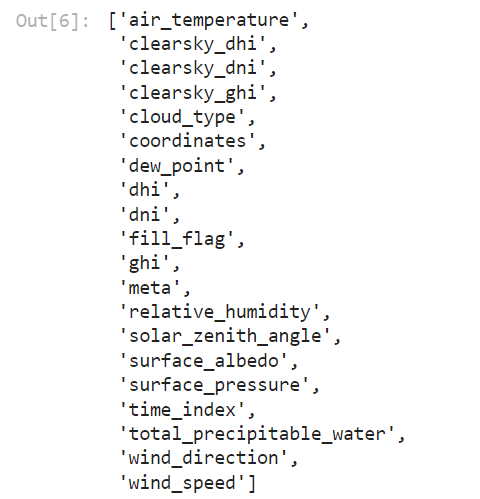
\includegraphics[width=0.3\textwidth]{Attrs}
    \caption{Attributes of a NSRDB dataset}\label{fig}
\end{figure}

\subsubsection{By using NSRDB web application }

NSRDB viewer on the NREL website can be used to get afore mentioned attribute values for a specific
location based on its latitude and longitude as we have DEM (digital elevation model) based on 
latitude and longitude this method would be preferred in this study.

\begin{figure}[h]
    \centering
    \begin{subfigure}{0.49\textwidth}
        \centering
        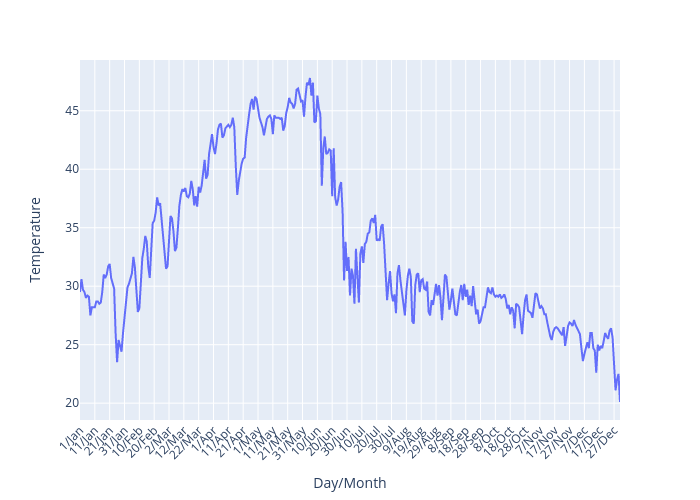
\includegraphics[width=1\textwidth]{Temperature}
        \caption{Temperature for coordinates N 20' E 78'}\label{fig:Temperature}
    \end{subfigure}
    \hfill
    \begin{subfigure}{0.49\textwidth}
        \centering
        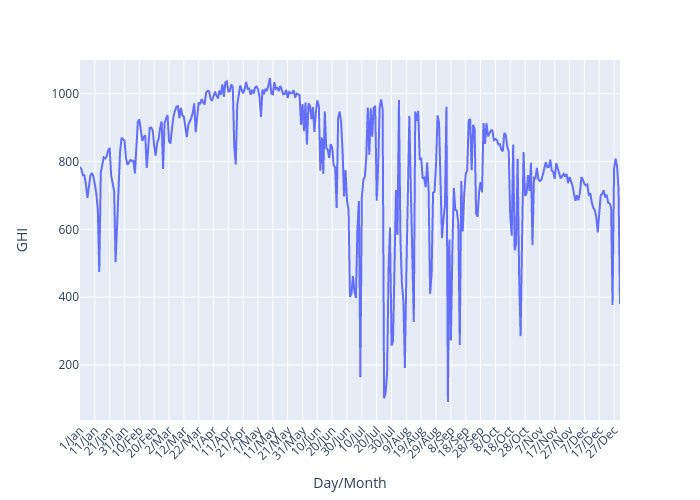
\includegraphics[width=1\textwidth]{GHI}
        \caption{GHI value by time }\label{fig: Global Horizonatal Irradiance}
    \end{subfigure}
    \hfill
    \begin{subfigure}{0.49\textwidth}
        \centering
        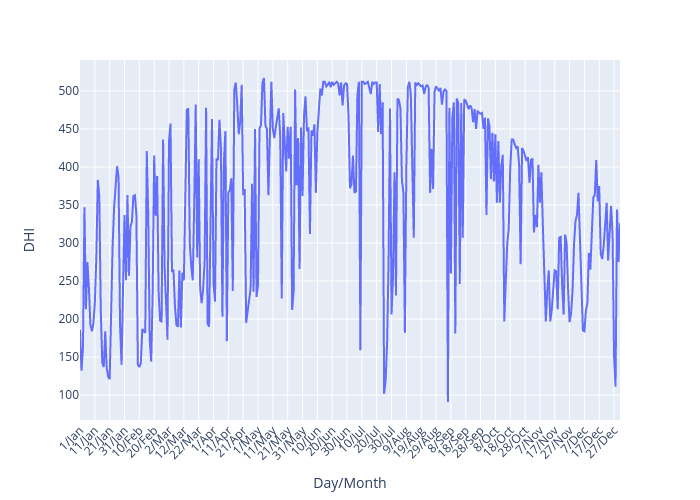
\includegraphics[width=1\textwidth]{DHI}
        \caption{DNI values by time}\label{fig: Direct Normal Irradiance}
    \end{subfigure}
    \caption{Comparison of Elevation and Elevation Data}
\end{figure}

\bibliographystyle{IEEEtranN}
\bibliography{biblography}
\end{document}